% Канонический TikZ-рисунок варианта 13. Править только здесь.
\newcommand{\figTangentialPerimeter}{%
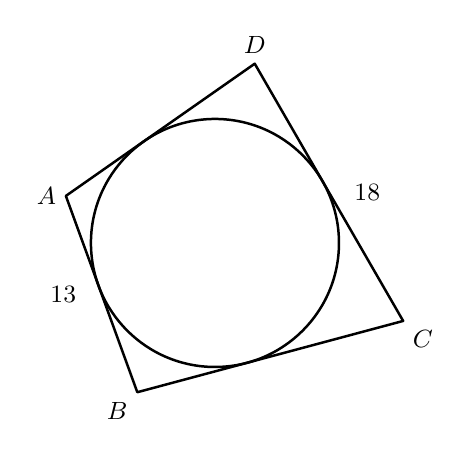
\begin{tikzpicture}[scale=1.05,line cap=round,line join=round,every node/.style={font=\small}]
  \coordinate (O) at (0,0);
  \coordinate (A) at (-1.803, 0.569); \coordinate (B) at (-0.939,-1.805);
  \coordinate (C) at ( 2.276,-0.943); \coordinate (D) at ( 0.481, 2.168);
  \draw[line width=0.9pt] (A)--(B)--(C)--(D)--cycle;
  \draw[line width=0.9pt] (O) circle (1.5);
  \path (A)--(B) node[midway,left=2mm] {$13$};
  \path (C)--(D) node[midway,right=2mm] {$18$};
  \node[left] at (A) {$A$}; \node[below left] at (B) {$B$};
  \node[below right] at (C) {$C$}; \node[above] at (D) {$D$};
\end{tikzpicture}}
